%%%%%%%%%%%%%%%%%%%%%%%%%%%%%%%%%%%%%%%%%%%%%%%%%%%%%%%%%%%%%%%%%
%                     swjtuThesis模板的主文件
%%%%%%%%%%%%%%%%%%%%%%%%%%%%%%%%%%%%%%%%%%%%%%%%%%%%%%%%%%%%%%%%%

\documentclass[oneside,openright]{swjtuThesis} % .cls文件
\usepackage{swjtuThesis} % .sty文件
% \usepackage{xxx,xxx,xxx,...} % 在.sty文件已导入了常见的必要宏包,如需额外添加请用户在此处添加!!!

% 加载论文信息,用户需要填写自己的信息!!!
%-------------------------------------------------------%
%                      中英文扉页信息
%-------------------------------------------------------%
% 论文类型
\cDegree{硕} % 硕士论文请填“硕”,博士论文请填“博”
\eDegree{Master} % 硕士论文请填“Master”,博士论文请填“Doctoral”
\eThesis{Thesis} % 硕士论文请填“Thesis”,博士论文请填“Dissertation”

% 论文标题
\cTitle{\underline{学~位~论~文~题~目}}
\eTitle{Thesis Template for Master Degree of \\ Engineering in \\
Southwest Jiaotong University}

% 国内图书分类号
\CI{TM30}
% 国际图书分类号
\UDC{621.3}
% 保密等级
\secLevel{公开}
% 单位代码
\UCode{10613}

% 专业
\cDiscipline{交通运输工程}
\eDiscipline{Transportation Engineering}
% 学号
\cStudentID{2024123456}
\eStudentID{2024123456}
% 作者姓名
\cAuthor{姜维} % 盲审使用:\cAuthor{\#\#\#}
\eAuthor{Wei Jiang} % 盲审使用:\eAuthor{\#\#\#}
% 导师姓名
% 请注意:如果需要加上导师职称,则导师姓名和导师职称之间加上\hspace{0.1em}以增大间距,整体显得更为美观,例如:诸葛亮 \hspace{0.1em} 副教授。 
\cSupervisor{诸葛亮} % 盲审使用:\cSupervisor{***}
\eSupervisor{Geliang Zhu} % 盲审使用:\eSupervisor{***}
% 学院
\cSchool{交通运输与物流学院}
\eSchool{School of Transportation and Logistics}
% 日期
\cDate{2024}{8}{10}
\eDate{2024}{Aug.}{10}

%---------------------------------------------------------------%
%                           前置部分
%---------------------------------------------------------------%

\makeatletter
\begin{document}

% 中英文扉页
\maketitlepage

% 独创性声明,注意电子版论文、纸质版论文的获取方法(参考README.md文件)!!!

\includepdf{01_frontPart/statement.pdf}

% 版权使用授权,注意电子版论文、纸质版论文的获取方法(参考README.md文件)!!!
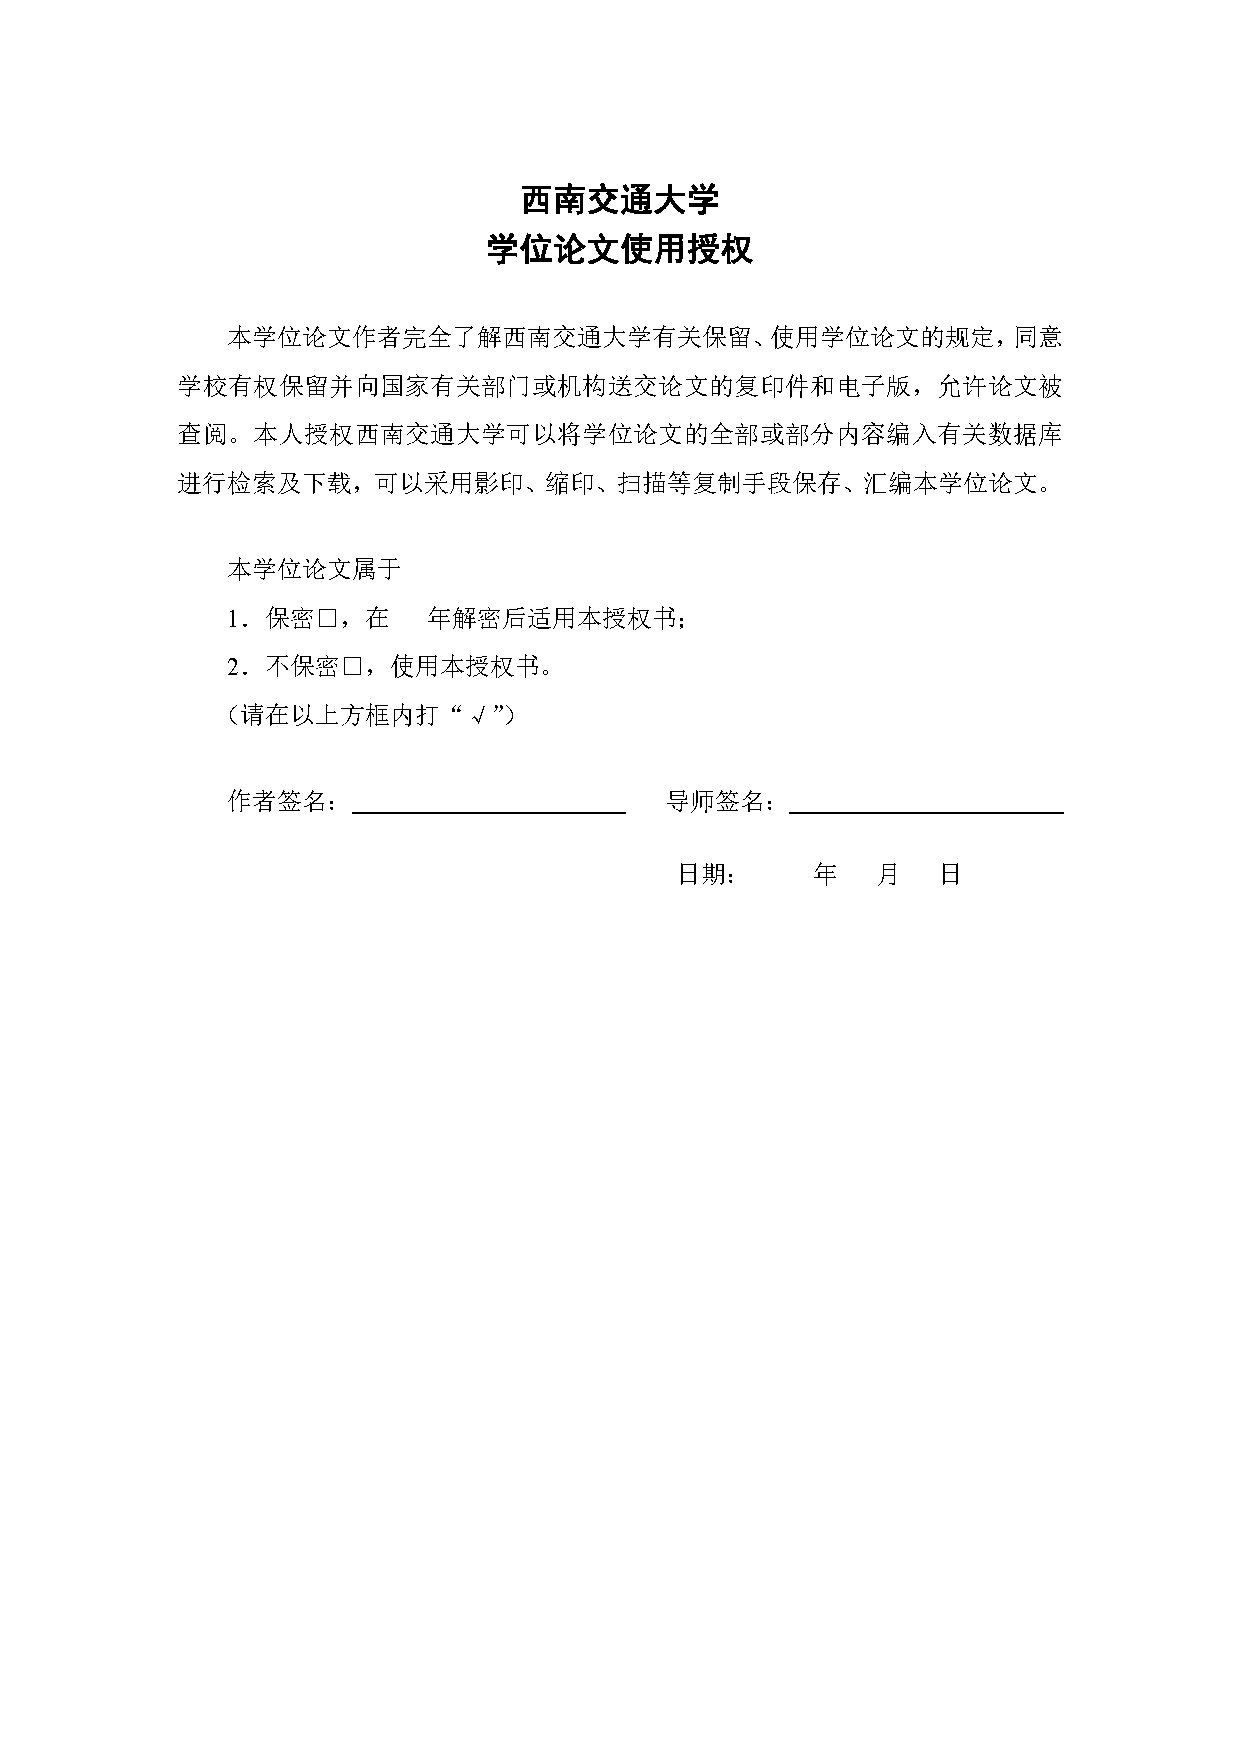
\includepdf{01_frontPart/copyright.pdf}

\setlength{\baselineskip}{20pt} % 从中文摘要开始,所有文字段落和标题行间距均取固定值20磅
\pagenumbering{Roman} % 从中文摘要开始,将页码设置成罗马数字并开始编号  

% 中英文摘要
%-------------------------------------------------------%
%                         中文摘要
%-------------------------------------------------------%
\chapter*{摘\quad 要}
\cabstractpagestyle % 中文摘要的页眉页脚

为进一步规范我校研究生学位论文撰写格式,提高研究生学位论文质量,参照国家标准《学术论文编写规则》(GB/T 7713.2-2022),结合我校实际,制定本范式。

相对于上一版的主要变化如下:

1. 按照最新范式重新编写文档,预置主要格式样式,可作为论文模板使用。

2. 更新摘要、绪论、正文、结论撰写说明,以及全文语言、表述注意事项。

3. 参照最新国家标准,调整参考文献格式要求。

4. 明确部分格式要求细节,如表格的样式,图表附注的格式,图表跨页等。

5. 附录增加西南交通大学研究生培养二级单位、常见一级学科中英文对照表以及西南交通大学专业学位类别。

此文档可在研究生院网站下载,如有变动,以研究生院网站最新公布的版本为准。

\vspace{1em}

\noindent \hangindent=3.9em \textbf{关键词:}学位论文,撰写格式,主要变化
%-------------------------------------------------------%
%                         英文摘要
%-------------------------------------------------------%
\chapter*{\textbf{ABSTRACT}}
\eabstractpagestyle % 中文摘要的页眉页脚

In order to further standardize the format of dissertation/thesis writing and improve graduate dissertation/thesis quality, this specification is formulated with reference to the national standard "Presentation of academic papers" (GB/T 7713.2-2022) and the reality of SWJTU.

The main changes in this revision from the last version are as follows.

1. Rewrite the document according to the requirements of the specifications, and preset main formatting styles, which can be used as a template directly.

2. Update the writing instructions of abstract, introduction, main chapters, and conclusions, as well as the notes on language and presentation.

3. Adjust the format requirements of references according to the latest national standards.

4. Clarify some details of format requirements, e.g., three-line style for tables, format for figure/table annotations, the problem of cross page figure/table.

5. Add comparison tables of Chinese and English names of colleges, academic degree disciplines, and professional degree categories in Appendixes.

This document can be downloaded from the Graduate School website. In case of any changes, the latest version published on the Graduate School website shall prevail.

\vspace{1em}

\noindent \hangindent=4.9em \textbf{Keywords: }Dissertation/Thesis, Writing Format, Main Changes

% 目录、图目录(如需)、表目录(如需)
\listpagestyle % 目录、图目录、表目录的页眉页脚
\tableofcontents
\listoffigures
\listoftables

% 主要符号表(如需)
%-------------------------------------------------------%
%                        主要符号表
%-------------------------------------------------------%
\chapter*{主要符号表}
\symbolpagestyle % 主要符号表的页眉页脚

\begin{longtable}{m{3em}m{0.7\textwidth}m{3em}}
% 表格第一页的标题
\textbf{符号} & \textbf{意义} & \textbf{单位}  \\
\endfirsthead
% 表格第二页的标题
\multicolumn{3}{c}
{续表\thetable 常见一级学科中英文名称对照表} \\
\textbf{代码} & \textbf{中文名称} & \textbf{英文名称}  \\
\endhead
$S_v$ & 空隙总面积 & $\mathrm{\mu m^2}$ \\
$\beta$ & 孔隙生长驱动力 &  \\

\end{longtable}

% 缩略词表(如需)
%-------------------------------------------------------%
%                         缩略词表
%-------------------------------------------------------%
\chapter*{缩略词表}
\acronympagestyle % 主要符号表的页眉页脚

\begin{longtable}{m{4em}m{0.6\textwidth}m{8em}}
% 表格第一页的标题
\textbf{英文缩写} & \textbf{英文全称} & \textbf{中文全称}  \\
\endfirsthead
% 表格第二页的标题
\multicolumn{3}{c}
{续表\thetable 常见一级学科中英文名称对照表} \\
\textbf{代码} & \textbf{中文名称} & \textbf{英文名称}  \\
\endhead
AUC & Area Under the Curve & 曲线下面积 \\
MLE & Maximum Likelihood Estimation & 极大似然估计 \\

\end{longtable}

\noindent 提示:为便于查阅,缩略词表按英文缩写字母顺序排序


%---------------------------------------------------------------%
%                           正文部分
%---------------------------------------------------------------%

\pagenumbering{arabic} % 从第1章第1页开始,将页码设置成阿拉伯数字并开始编号
\mainpagestyle % 从第1章第1页及之后的部分的页眉页脚

% 绪论、具体研究内容、结论
%-------------------------------------------------------%
%                        第1章内容
%-------------------------------------------------------%
\chapter{基本结构及主要内容}\label{第1章}

\section{基本结构}

学位论文包括前置部分、正文部分和结尾部分共三大部分,各部分组成及顺序如图\ref{fig:学位论文基本结构}所示。

\begin{figure}[h]
    \centering
    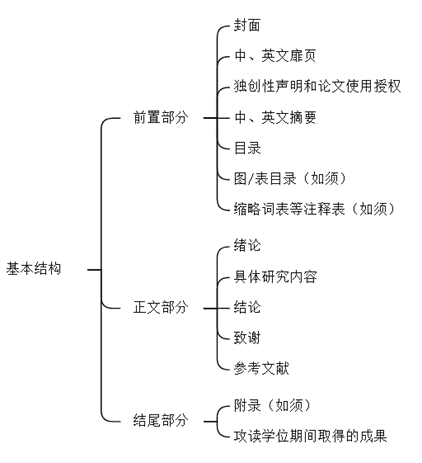
\includegraphics[width=0.7\linewidth]{figures/figure1.png}
    \caption{学位论文基本结构}
    \label{fig:学位论文基本结构}
\end{figure}

\section{前置部分}

\subsection{封面}

不同学位类别对应不同封面。其中,博士学位封面分为精装本、简装本,精装本为绿色漆布材质,烫金字体;硕士学位只有简装本。

论文题目是论文的总纲,是反映论文中重要特定内容的恰当、简明的词语的逻辑组合。题名用词须考虑有助于选定关键词和编制题录、文摘等二次文献所需的使用信息,力求简短,\textbf{避免使用不常用的缩略词、首字母缩写字、字符、代号、公式等,一般不宜超过25字}。

如题名内容层次很多,难以简化时,可采用题名和副题名相结合的方法,副题名起补充、阐明题名的作用。中文的题名与副题名之间用破折号相连,英文则用冒号相连。题名和副题名在整篇学位论文中的不同地方出现时,应保持一致。

指导教师:以研究生管理信息系统登记的责任导师为准,且\textbf{只能填写一名指导教师}。

\subsection{扉页}

学科专业:参照研究生管理信息系统登记的学科专业,以国务院学位委员会批准的学科目录为准。其中,学术学位研究生:按学科目录一级学科培养的,填一级学科;按学校自主设置二级学科培养的,填所属一级学科;按学科目录二级学科培养的,填二级学科。

指导教师:以研究生管理信息系统登记的责任导师为准,若还有其他导师联合指导,可一起填写在扉页,中间用顿号隔开(指导教师最多填2位)。

\textbf{涉密学位论文},按学校相关规定,还须在封面右上角按“密级$\bigstar$保密期限”格式标注,例如“秘密$\bigstar$10年”。

\subsection{独创性声明和论文使用授权}

内容、样式及填写说明见本文档开头部分。除提交盲审的学位论文外,导师及研究生本人须在独创性声明和论文使用授权相应位置签字。

\subsection{摘要}

摘要是学位论文内容不加注释和评论的简短陈述。摘要应具有独立性和自含性,是一篇简短但意义完整的文章,内容应包括研究目的、内容、方法、结果和结论等,\textbf{重点是结果、结论}。

摘要的内容要完整、客观、准确,应做到不遗漏、不拔高、不添加,按层次逐段简要写出。摘要在叙述研究内容、研究方法和主要结论时,除作者的价值和经验判断可以使用第一人称外,一般使用第三人称,采用“分析了……原因”“研究了……”“对……进行了探讨”“给出了……结论”等记述方法进行描述。避免主观性的评价意见,避免对背景、目的、意义、概念和一般性(常识性)理论叙述过多。

摘要需采用规范的名词术语(包括地名、机构名和人名)。对个别新术语或无中文译文的术语,可用外文或在中文译文后加括号注明外文。摘要中应尽量避免使用图、表、化学结构式、非公知公用的符号与术语,不标注引用文献编号。

硕士论文中文摘要\textbf{一般不超过800字,且篇幅控制在1页以内};博士论文中文摘要\textbf{一般不超过1500字,篇幅控制在2页以内}。英文摘要另起一页书写,标题ABSTRACT全部大写,内容与中文摘要一致,翻译准确,博士论文译为“Dissertation”,硕士论文译为“Thesis”。

\subsection{关键词}

关键词是用以表示全文主题内容信息的单词或术语,一般为3~8个。关键词应体现论文特色,具有语义性,在论文中有明确的出处,不应使用太泛指的词,例如“方法”、“理论”、“分析”等。

应尽量采用《汉语主题词表》或各专业主题词提供的规范词。与摘要正文之间空一行顶格书写,用\textcolor{red}{逗号}隔开。若关键词超过一行,换行后应悬挂缩进对齐。英文关键词应与中文关键词对应,每个单词首字母大写。

\subsection{目录}

目录是论文的提纲。\textbf{目录内容从“第1章”开始}至论文最后一页,包含论文正文部分的全部章、节、条三级标题及其起始页码,排在序言或前言之后,另起页。

\subsection{图/表目录}

如果论文中使用了大量的图片或表格,可分别列出索引清单置于目录之后。

图的清单应有序号、图题和页码,表的清单应有序号、标题和页码,样式见本文档图目录。

\subsection{注释表}

如果论文中使用了大量的符号、标志、缩略词、计量单位、自定义名词和术语等,应编写成注释表汇集表置于目录之后。若上述符号使用数量不多,可以不设此部分,但必须在论文中初次出现是加以说明。

符号、缩略词等注释表样式见本文档主要符号表、缩略词表。

\section{正文部分}

正文部分是学位论文的主题和核心部分,一般从绪论开始,包括具体研究内容、结论、参考文献等,应层次分明、逻辑性强。

\subsection{绪论}

绪论(第1章)应简要阐明论文的选题,选题背景及意义,国内外相关研究成果与进展述评,存在的不足或有待进一步研究的问题,本论文所要解决的科学与技术问题、所运用的主要理论和方法、基本思路和论文结构等。

绪论要注意对论文所引用的国内外文献进行准确标注。

\subsection{具体研究内容}

具体研究内容是论文的主要部分,根据学科专业特点和选题情况,可以有不同的写作方式,但应遵循本学科通行的学术规范,必须实事求是,客观真切,准确完备,合乎逻辑,层次分明,重点突出,文字简练、通顺。

学位论文应围绕一个主题,针对某学科领域中的一个具体问题展开深入、系统的研究,并得出有价值的研究结论。论文各章之间应该前后关联,构成一个有机整体。论文给出的数据必须真实可靠,推理正确,结论明确,无概念性和科学性错误。对于科学实验、计算机仿真的条件、实验过程、仿真过程等需加以叙述,然后对结果进行分析及理论提升,避免直接给出结果、曲线和结论。引用他人研究成果或采用他人成果时,应注明出处,不得将其与本人提出的理论分析混淆在一起。

论文各章末尾应有“本章小结”,实验方法或材料等章节可不写“本章小结”。各章小结是对各章研究内容、方法与成果的简洁准确的总结与概括,也是论文最后结论的依据。

\subsection{结论}

结论(最后1章)是论文总体的、最终的结论,并不是各章小结的简单重复,应精炼、准确、完整。结论应包括论文的核心观点,重点阐述论文的创造性工作和创新性成果,及其在本领域内的地位、作用和意义,说明论文研究工作的局限或有待进一步研究和探讨的问题,提出未来工作的设想或建议。

\subsection{致谢}

致谢对象包括资助研究工作的基金、组织或个人,协助完成研究工作的组织或个人,在研究工作中提出重要建议或提供重要帮助的组织或个人以及提供转载和引用权的资料、图片、文献、研究思想和设想的所有者等,\textbf{一般不超过800字}。

\subsection{参考文献}

参考文献应置于正文后,并另起页。

学位论文的撰写应本着严谨求实的科学态度,所有被引用文献均要列入参考文献中,必须按文中出现的顺序标注,但同一篇文献只用一个序号。

尽量引用原始文献。当不能引用原始文献时,要将二次引用文献、原始文献同时标注。\textcolor{red}{博士学位论文的参考文献一般不少于100篇,学术型硕士学位论文的参考文献一般不少于50篇,专业硕士学位论文的参考文献一般不少于30篇,其中外文文献一般不少于总数的1/2}。参考文献中近五年的文献数一般应不少于总数的1/3,并应有近两年的参考文献和一定数量的学位论文或专业名著。

产品说明书、未公开发表的研究报告(著名的内部报告如PB、AD报告及著名大公司的企业技术报告等除外)以及其它无法通过公开途径获得的文献资料通常不宜作为参考文献引用。

引用网上参考文献时,应注明该文献的准确网页地址,网上参考文献和各类标准不包含在上述规定的文献数量之内。\textbf{本人在攻读学位期间发表的学术论文不应列入参考文献中},具体格式要求见\ref{sec2.9}节。

\section{结尾部分}

\subsection{附录}

附录是作为论文主体的补充项目(非必须),主要包括正文内不便列出的冗长公式推导、某些重要的原始数据、计算程序及说明等。文中的附录A、B、C仅供做参考,不出现在正文中。

\subsection{攻读学位期间取得的研究成果}

在攻读博士(硕士)学位期间取得的与论文内容相关的研究成果,例如:发表和已录用的学术论文、专著/译著、参与的科研项目、专利、作品、科研获奖等。与学位论文无关的学术论文不宜在此列出,具体格式要求见\ref{sec2.10}节。

\section{各部分标题英文翻译}

用英文撰写的学位论文,内容、格式要求与中文学位论文一致。各部分标题中英文翻译对照如\ref{tab1-1}所示。

\begin{table}[!ht]
\centering
\caption{学位论文各部分标题中英文翻译对照表}
\label{tab1-1}
\begin{tabularx}{\textwidth}{ 
>{\centering\arraybackslash}X 
>{\centering\arraybackslash}X
}
\toprule
中文 & 英文 \\
\midrule
摘要 & ABSTRACT \\
目录 & Contents \\
图目录 & Figures \\
表目录 & Tables \\
主要符号表 & Symbols \\
缩略词表 & Acronyms \\
参考文献 & References \\
致谢 & Acknowledgements \\
附录(附录A,附录B......) & Appendix (Appendix A, Appendix B...) \\
\bottomrule
\end{tabularx}
\end{table}

\section{本章小节}

本章主要对学位论文的基本结构和主要内容进行了详细说明。
%-------------------------------------------------------%
%                        第2章内容
%-------------------------------------------------------%
\chapter{格式规范}\label{第2章}

\section{语言和表述}

研究生学位论文要求用汉语书写,所用汉字须符合教育部、国家语言文字工作委员会组织制定的《通用规范汉字表》。专用名词、术语可采用国际通用的代号,量及其单位所使用的符号应符合国家标准《国际单位制及其应用》(GB3100—1993)、《有关量、单位和符号的一般原则》(GB/T 3101—1993)的规定。图、表中的图题、坐标轴、图例、表头等描述性的词组或语句须使用汉语,专用名词术语、物理量及其单位可使用符合规范要求的符号。

根据教育部、外交部、公安部联合制定的《学校招收和培养国际学生管理办法》(教育部令第42号)有关规定,使用外国语言接受高等教育学历的国际学生,其学位论文可使用相应的外文撰写,但须附\textcolor{red}{5000}字的详细中文摘要,并放在英文摘要之前。

学位论文表述要严谨简明,重点突出,专业常识应简写或不写,做到立论正确、层次分明、数据可靠、文字凝练、说理透彻、推理严谨,避免使用文学性质的带感情色彩的非学术性词语。\textbf{学位论文作者具有唯一性,避免“我们”等用词}。

\section{标题和层次}

论文各章节标题要突出重点、简明扼要,尽量控制在一行,标题中不加标点符号。标题中尽量不采用英文缩写词,必须采用时应使用本行业的通用缩写词。

论文章节层次要清楚,\textbf{一般到三级层级(例如“1.1.1”)即可},最多到四级层次。各章节层次均应有标题,标题由序号和名称组成,之间空1个汉字符。一级标题(章标题)居中书写,次级标题顶格书写。

\section{字体和段落}

\textbf{若无特殊说明,论文中的中文统一用宋体,数字和英文统一用Times New Roman字体。从中文摘要开始,所有文字段落和标题行间距均取固定值20磅;所有段落按两端对齐、首行缩进2个汉字符方式书写内容。}

\textbf{中文用黑体或加粗的地方,对应数字和英文宜使用加粗Times New Roman字体。}

中、英文字号对应关系如表\ref{tab2-1}所示,主要文字及段落格式要求如表\ref{tab2-2}所示。


\begin{table}[!ht]
\centering
\caption{中、英文字号对应关系}
\label{tab2-1}
\begin{tabularx}{\textwidth}{ 
>{\centering\arraybackslash}X 
>{\centering\arraybackslash}X
>{\centering\arraybackslash}X
>{\centering\arraybackslash}X
}
\toprule
\textbf{中文字号} & \textbf{英文磅数} & \textbf{中文字号} & \textbf{英文磅数} \\
\midrule
二号 & 22 & 四号 & 14 \\
小二 & 18 & 小四 & 12 \\
三号 & 16 & 五号 & 10.5 \\
小三 & 15 & 小五 & 9 \\
\bottomrule
\end{tabularx}
\end{table}

\begin{table}[!ht]
\centering
\caption{主要文字及段落格式要求}
\label{tab2-2}
\begin{tabular}{ccccccm{0.3\textwidth}}
\toprule
\textbf{内容} & \textbf{字体} & \textbf{字号} & \textbf{对齐方式} & \textbf{段前距} & \textbf{段后距} & \textbf{备注} \\
\midrule
一级标题 & 黑体 & 三号 & 居中 & 24磅 & 18磅 &  \\
二级标题 & 黑体 & 四号 & 顶格左对齐 & 18磅 & 6磅 &  \\
三级标题 & 黑体 & 四号 & 顶格左对齐 & 12磅 & 6磅 &  \\
四级标题 & 黑体 & 小四 & 顶格左对齐 & 12磅 & 6磅 &  \\
正文 & * & 小四 & 两端对齐 & 0磅 & 0磅 & \footnotesize{*未注明字体的,统一按“中文宋体,英文、数字Times New Roman”原则} \\
 &  &  & (首行缩进) &  &  &  \\
页眉 &  & 五号 & 居中 & 0磅 & 0磅 &  \\
页码 &  & 小五 & 居中 & 0磅 & 0磅 &  \\
脚注 &  & 小五 & 两端对齐 & 0磅 & 0磅 &  \\
参考文献 &  & 五号 & 两端对齐 & 0磅 & 0磅 &  \\
 &  &  & (悬挂缩进) &  &  &  \\
附录 &  & 五号 & * & 0磅 & 0磅 & \footnotesize{*根据附录形式选择合适的排版方式。} \\
图片 &  & 五号* & 居中 & 6磅 & 0磅 & \footnotesize{*图中文字显示大小跟图题文字一致。} \\
图题 &  & 五号 & 居中* & 6磅 & 12磅 & \footnotesize{*超过一行的图题并非居中,详见\ref{sec2.4.1}} \\
表格 &  & 五号 & 居中 & 0磅 & 6磅 & \footnotesize{一般采用三线表样式} \\
表题 &  & 五号 & 居中* & 12磅 & 6磅 & \footnotesize{*超过一行的表题并非居中,详见\ref{sec2.4.2}} \\
图表附注 &  & 五号 & 顶格 & 6磅 & 6磅 &  \\
公式 &  & 小四 & 居中 & 6磅 & 6磅 &  \\
公式编号 &  & 小四 & 右对齐* & 6磅 & 6磅 & \footnotesize{*公式编号前不加引导线,详见\ref{sec2.5}} \\
\bottomrule
\end{tabular}
\end{table}

其他要求:

1. 各级标题不得置于页面的最后一行,即须与下段同页;

2. 两个标题之间无正文时,第二个标题的段前距设置为0磅;

3. 图、表、公式统一采用单倍行距;

4. 只有一、两行文字的,不得单独作为一页内容;

5. 除各章最后一页外,中间页面不得出现较大空白;

6. 必要时,可在规定的格式要求基础上适当微调,以利于排版,但显示效果不得与规定的格式要求存在明显差距。

\section{图表}

图、表和表达式应居中放置,按章编号,用两位阿拉伯数字分别编号,前一位数字为章的序号,后一位数字为本章内图、表或表达式的顺序号,两个数字中间用短横线连接,如“图1-4”、“表1-2”,“式(3-5)”。在图、表紧邻的前文中,须有相应提示,例如“如图1-2所示”“见表1-3”等。若图或表中有附注,采用英文小写字母顺序编号,附注写在图或表的下方。

引用文献中的图、表时,除在正文文字中标注参考文献序号以外,还须在\textbf{图题、表题的右上角标注参考文献序号}。

\subsection{图}\label{sec2.4.1}

图要求精练,具有“自明性”,即只看图、图题和图例,不阅读正文,就可理解图意。作图须符合相关标准或行业惯例;图片清晰、易于分辨,能满足复印、微缩需要;图中的术语、符号、单位等应与正文表述中一致。

每个图应有\textbf{图序、图题},五号\textcolor{red}{宋体},单倍行距,居中置于图的下方,段前距6磅,段后距12磅,图序与图题文字之间空1个汉字符的宽度;超过一行时,两端对齐,左右缩进4字符。若有分图,\textbf{分图题置于主图题之后};分图序号用 (a)、(b)、(c)等表示,五号\textcolor{red}{宋体},居中置于对应分图正下方,也可置于对应分图左上角等位置,但应全文统一,如图\ref{fig:有分图的情况的示例}。若有附注,用五号字顶格写在图题下方,首段段前距、末段段后距设为6磅。

\begin{figure}[!ht]  
    \centering
    \begin{subfigure}[t]{0.45\textwidth}
        \centering
        
\includegraphics[width=\linewidth]{example-image-a.pdf}
        \caption{}
    \end{subfigure}
    \quad
    \begin{subfigure}[t]{0.45\textwidth}
        \centering
        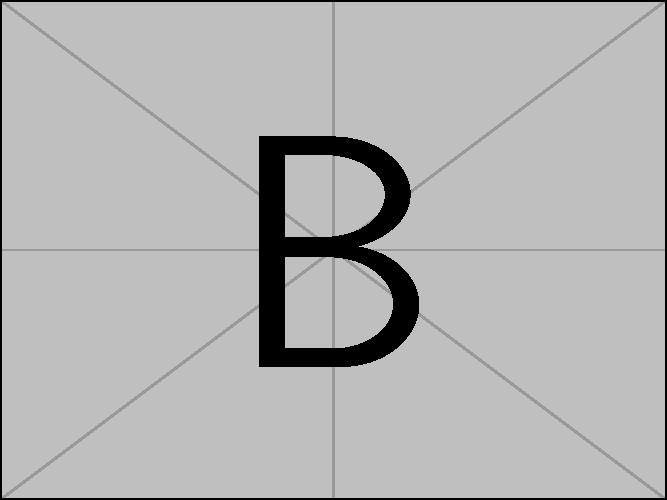
\includegraphics[width=\linewidth]{example-image-b.pdf}
        \caption{}
    \end{subfigure}
    \caption{分图题置于主图题之后:(a)分图一的标题;(b)分图二的标题}
    \label{fig:有分图的情况的示例}
\end{figure}

\textbf{图中文字显示大小应与图题文字大小一致}。若非直接引用的图,除缩略词、单位外,图中坐标轴、说明性文字等应\textbf{统一使用中文}。

\textbf{图和图题须编排在同页,图题不得跨页}。如图太宽,可逆时针方向旋转90°放置。图页面积太大时,可分别配置在两页上,次页需注明“续”字,并注明图题,如“续图1-1 高光谱遥感技术成像示意图”。如需英文图名,应中英文对照,英文序号与内容应与中文一致,在中文下方另起一行。

\subsection{表}\label{sec2.4.2}

表应有“自明性”。表中参数应标明量和单位的符号。为使表格简洁明了,\textcolor{red}{均}采用\textbf{三线表}(必要时可加辅助线,三线表无法清晰表达时可采用其他格式),表的上下边线为单直线,线粗1.5磅,第三条线为单直线,线粗1磅。

每个表应有\textbf{表序、表题},五号\textcolor{red}{宋体},单倍行距,居中置于表的上方,段前距12磅,段后距6磅;表序与表题文字之间空1个汉字符的宽度;超过一行时,两端对齐,左右缩进4字符。表题的表格之后首段正文的段前距6磅。若有附注,用五号字顶格写在表下方,首段段前距、末段段后距设为6磅。

表单元格中的文字一般应居中书写(上下居中、左右居中),不宜左右居中书写的,可采用两端对齐的方式书写;五号宋体、单倍行距、段前空3磅,段后空3磅。

\textbf{表格一般不跨页编排},仅当一页内编排不下时才可转页,以续表形式接排,格式同前,续表均应重复表头,并在每页表序前加“续”字,如“续表2-3 不同主成分分量取值(K)对两个模型分类精度的影响情况(\%)”。

\section{公式}\label{sec2.5}

公式主要是指数学表达式,例如数学公式,也包括文字表达式。公式一般另起一行居中书写,采用与正文相同的字号,或另起一段空两个字符书写,全文须使用统一采用某一种格式。公式应有序号,序号加括号置于公式所在行\textbf{最右端,不加任何连线}。在公式紧邻的前文中,须有相应提示,例如“见式(1-2)”等。

较长的表达式必须转行时,应在“=”或者“+”“-”“×”“/”等运算符或者“]”“\}”等括号之后回行。上下行尽可能在“=”处对齐。例如:
\begin{equation}
    \begin{aligned}
    x&=1+2\\
     &=3
    \end{aligned}
\end{equation}

公式采用Cambira Math或Times New Roman字体,\textbf{单倍行距},段前、段后距均为6磅。
当公式不是独立成行书写时,应尽量将其高度降低为一行,例如,将分数线书写成“/”,将根号改为负指数,例如$8^{-1/2}$。

\section{量和单位}

严格执行《量和单位》国家标准(GB 3100-93)、GB/T 3101-93、GB/T 3102.1~13-93等共15项)有关量和单位的规定。计量单位书写,可以采用国际通用符号,也可以用中文名称,但\textbf{全文应统一},不得两种混用;以人名命名的计量单位首字母大写。

\textbf{量的符号采用斜体书写,计量单位用正体书写};量与单位间用斜线隔开,例如:$I/\mathrm{A}$,$\rho/\mathrm{kg \cdot m^{-3}}$,$F/\mathrm{N}$,$v/\mathrm{m \cdot s^{-1}}$等。

不定数字之后允许使用中文计量单位符号,如“几千克”;非中文数值和计量单位之间空\textbf{1个字符},例如“1 m”。表达时刻时应采用中文计量单位,如“上午8点1刻”,不能写成“8h15min”。

\section{标点符号和数字}

执行国家标准《标点符号用法》(GB/T15834-2011)和《出版物上数字用法》(GB/T 15835-2011)相关规定。除习惯用中文数字表示的以外,一般数字统一用阿拉伯数字。

\section{脚注}

脚注是对论文中某一特定内容所做的进一步解释或补充说明,相关内容切忌直接在文中注释,一般放在该页地脚。脚注序号用阿拉伯数字加圆圈按页编排,每页的脚注序号均从“\textcircled{1}”开始,采用非“上标”样式,与脚注内容之间空半个汉字符。脚注用小五号字,单倍行距,两端对齐,悬挂缩进1.5字符。

\section{参考文献}\label{sec2.9}

参考文献应具有权威性和时效性,列示须实事求是,\textbf{引用过的文献必须著录,未引用的文献不得虚列}。文献标注及书写格式执行国家标准《信息与文献 参考文献著录规则》(GB/T 7714-2015)相关规定。

\subsection{文献引用标注}

1. 采用顺序编码制,按正文中引用文献出现的先后顺序连续编码,并将序号置于方括号“[ ]”中,以上标方式标注在引用位置;

2. 同一处引用多篇文献,应将各篇文献的序号在方括号“[ ]”中全部列出,各序号间用逗号,如遇连续序号,起讫序号间用短横线“-”连接,例如“通过提取地物目标可分性更好的空谱特征来实现其有效分类[65, 66, 70-77]”;

3. 作为句子有效成分的引用标志不用上标,如“由文献[4, 7-10]可知”;

4. 重复引用同一文献,始终标注第一次引用的序号;

5. 除引用的图表标题外,不得将引用文献引用标注置于各级章节标题处。

\subsection{文献书写格式}

参考文献使用\textbf{五号字}。常见参考文献书写格式如表\ref{tab2-3}所示。


\begin{table}[!ht]
\centering
\caption{常见参考文献书写格式}
\label{tab2-3}
\begin{tabular}{m{4em}<{\centering}m{0.85\textwidth}<{\raggedright}}
\toprule
文献类型 & 书写格式 \\
\midrule
期刊论文 & [序号] 作者. 文章题目[J]. 期刊名, 年, 卷(期): 起-止页码. \\
会议论文 & [序号] 作者. 题名[C]. 会议名, 会议地, 会议年: 起-止页码. \\
专著 & [序号] 作者. 书名[M]. 译者. 版本. 出版地: 出版者, 出版年: 起-止页码. \\
学位论文 & [序号] 作者. 题名[D]. 授位单位所在地: 授位单位, 授位年: \textcolor{red}{起-止页码}. \\
报纸文章 & [序号] 作者. 题名[N]. 报纸名, 出版日期 (版面数). \\
报告 & [序号] 作者. 题名[R]. 出版地: 出版者, 出版年.\\
专利 & \hangindent=3em [序号] 专利申请者或所有人. 专利题名[P]. 专利国别, 专利号. 公告日期或公开日期. \\
标准 & [序号] 发布单位. 标准名: 标准号[S]. 出版地: 出版者, 出版年: 起-止页码. \\
电子文献 & \hangindent=3em [序号] 作者. 题名[文献类型标识/文献载体标识]. 出版地: 出版者, 出版年: 起-止页码 (更新或修改日期) [引用日期]. 获取或访问路径. 数字对象唯一标识符.\\
\bottomrule
\end{tabular}
\end{table}

说明:

1. 参考文献\textbf{不跨页编排},即一条文献所在段中不分页;

2. 参考文献\textbf{悬挂缩进、两端对齐},所有\textbf{文献编号左侧对齐},文献编号和文献内容之间统一\textcolor{red}{空}2.5\textcolor{red}{个字符(模版已设置)},所有\textbf{文献内容左侧对齐};

3. 作者\textbf{姓在前、名在后,英文姓全拼、首字母大写,英文名大写缩写且不加点},例如“Harrington R F”(Roger F. Harrington),“Li M”(Li Moumou);

4. 作者姓名之间用逗号隔开,\textbf{最多写到第3位作者},余者用“, 等”或“, et al.”代替;

5. 除特殊名词外,\textbf{英文文献标题(论文题目、书名)仅第一个单词的首字母大写},其余全部小写;\textbf{英文文献出处(期刊名、会议名等)一般每个单词的首字母大写},只有长度为1~4字母的虚词全部小写,例如“in”“with”;

6. 日期统一用8位数字“YYYY-MM-DD”格式,年、月、日用短横线隔开;

7. 若文献本身不具备个别著录要素,则不著录该要素及对应的标识符号,例如,没有期号的期刊论文,其格式书写为“[序号] 作者. 文题[J]. 期刊名, 年, 卷: 起-止页码.”;

8. 初版的专著不著录版本,电子文献数字对象唯一识别符仅在获取或访问路径中不含数字对象唯一识别符时著录。

常见文献类型及标识代码见表\ref{tab2-4},电子资源载体及标识代码见表\ref{tab2-5}。\textbf{参考文献实例见第\textcolor{red}{20}页}。


\begin{table}[!ht]
\centering
\caption{文献类型和标识代码}
\label{tab2-4}
\belowrulesep=0pt % 三线表的中间的辅助线
\aboverulesep=0pt
\begin{tabularx}{\textwidth}{ 
>{\centering\arraybackslash}X 
>{\centering\arraybackslash}X|
>{\centering\arraybackslash}X
>{\centering\arraybackslash}X
}
\toprule
参考文献类型 & 标识代码 & 参考文献类型 & 标识代码 \\
\midrule
普通图书 & M & 专利 & P \\
会议录 & C & 数据库 & DB \\
汇编 & G & 计算机程序 & CP \\
报纸 & N & 电子公告 & EB \\
期刊 & J & 档案 & A \\
学位论文 & D & 舆图 & CM \\
报告 & R & 数据集 & DS \\
标准 & S & 其他 & Z \\
\bottomrule
\end{tabularx}
\end{table}

(图书例如\cite{杨新文2017轨道交通轮轨噪声机理预测与控制,教育部国家语言文字工作委员会2018通用规范汉字表,霍夫斯基主编1981禽病学,王夫之1865宋论,白书农1998植物开花研究,Itkis1976control});标准例如\cite{全国信息与文献标准化技术委员会2007学位论文编写规};专利例如\cite{姜锡洲1983一种温热外敷药制备方案,王士民2023一种用于研究盾构隧道管片上浮形态的模型实验装置};期刊例如\cite{高晗2020深度学习模型压缩与加速综述,zeng2019spectrum,rathgeb2023extended};学位论文例如\cite{陈梦玉2021基于人工智能算法的无线网络认知通信信号波形技术研究};报纸例如\cite{仲音2023敢做善为抓落实};报告例如\cite{冯西桥1997核反应堆压力容器的LBB分析};自定义例如\cite{萧钰2001出版业信息化驶入快车道}。

\begin{table}[!ht]
\centering
\caption{电子资源载体类型和标识代码}
\label{tab2-5}
\belowrulesep=0pt
\aboverulesep=0pt
\begin{tabularx}{\textwidth}{ 
>{\centering\arraybackslash}X|
>{\centering\arraybackslash}X
}
\toprule
电子资源的载体类型 & 载体类型标识代码 \\
\midrule
磁带(magnetic tape) & MT \\
磁盘(disk) & DK \\
光盘(CD-ROM) & CD \\
联机网络(online) & OL \\
\bottomrule
\end{tabularx}
\end{table}

\section{攻读学位期间取得的研究成果}\label{sec2.10}

攻读学位期间取得的研究成果只列出在攻读博士(硕士)学位期间取得的\textbf{与学位论文内容密切相关、能反映学位论文研究工作}的研究成果,例如发表和已录用的学术论文、专著/译著、参与的科研项目、专利、作品、科研获奖等。书写格式如下:

1. 学术论文书写格式与参考文献基本一致,尚未刊载但已收到正式录用函的学术论文加括号注明已被***期刊录用;

2. 专著/译著尚未出版但已被出版社决定出版的专著/译著加括号注明出版社名称和预计出版时间;

3. 专利书写格式与参考文献基本一致,处于\textcolor{red}{申请阶段}的专利在专利位置填写专利申请号,并加括号注明是专利申请号;

4. 作品大致书写格式:作者. 作品名称. 创作时间. 材料形式. 作品尺寸. 作品地点. 参展信息. 是否获奖等信息;

5. 科研获奖大致书写格式:获奖人. 项目名称. 获奖名称及等级, 发奖机构, 获奖日期;

6. 公开的研究报告书写格式与参考文献基本一致;

7. 未列举的其他类型成果,可参照上述格式要求书写;

8. \textbf{本人姓名加粗},列出所有作者,若作者超过5人,也可按“本人姓名(本人排名次序/总人数)”格式代表所有作者。

\section{页面设置、页眉和页码}

\subsection{页面设置}

博士学位论文和硕士学位论文除“中文封面”、“英文封面”、“学位论文指导小组、公开评阅人、和答辩委员会名单”和“学位论文独创性声明、学位论文使用授权”等四部分采用单面印刷外,从中文摘要开始后面的部分均采用A4幅面白色70克以上80克以下(彩色插图页除外)双面印刷,正文从另页右页开始。页面设置数据如下:

页边距:上—3.0厘米,下—3.0厘米,左—3.0厘米,右—3.0厘米,装订线0厘米;

页码范围:普通

页眉距边界:2厘米,页脚距边界:2厘米。

\subsection{页眉}

论文除中文摘要之前的前置部分(封面,中、英文扉页,独创性声明及论文使用授权页)不编排页眉外,其余页面均须编排页眉。

页眉采用\textbf{五号字}居中书写,中文用宋体,英文和数字用Times New Roman体;页眉线为单横线,线宽0.75磅。

中文摘要及之后的前置部分,页眉为各部分内容的标题,例如:“摘要”“ABSTRACT”“目录”“图目录”“表目录”“主要符号表”“缩略词表”。从第1章第1页开始,至论文最后一页,\textcolor{red}{\textbf{页眉统一用“西南交通大学博/硕士学位论文”}}。

\subsection{页码}

页码位于页面底端居中书写,\textbf{小五号字},Times New Roman体,页码数字两侧不加“-”等修饰线。

中文摘要及之后的\textbf{前置部分}(中、英文摘要,目录,图目录,表目录,主要符号表、缩略词表等注释表),\textbf{用大写罗马数字}“\uppercase\expandafter{\romannumeral1}、\uppercase\expandafter{\romannumeral2}、\uppercase\expandafter{\romannumeral3}......”从 “\uppercase\expandafter{\romannumeral1}”开始连续编排页码。从正文“第1章”(“引言”、绪论)开始,至论文最后一页,用\textbf{阿拉伯数字}“1、2、3......”从“1”开始连续编排页码。

\section{书脊}

\textcolor{red}{书脊信息应包括:获取学位年份、学位等级、学位论文中文题目、学生姓名、西南交通大学三部分(学位论文中文题目、学生姓名请用相应内容覆盖)。}

\textcolor{red}{中文四号黑体,英文、数字、字母等采用三号Times New Roman字体。论文题目距离顶端2厘米。}

\section{本章小结}

本章主要讲述了学位论文的具体格式范式。

\textbf{涉密学位论文的印刷、制作、传递、存档等,须符合国家、学校相关保密要求。} 
%-------------------------------------------------------%
%                        第3章内容
%-------------------------------------------------------%
\chapter{印制要求}\label{第3章}

\section{论文装订}

学位论文一律左侧装订。

装订时严格按照以下顺序排列:

\begin{enumerate}
    \item 论文封面
    \item 论文中、英文扉页
    \item 西南交通大学学位论文独创性声明
    \item 西南交通大学学位论文使用授权
    \item 中文摘要
    \item 英文摘要
    \item 目录
    \item 图/表目录(如须)
    \item 缩略词等注释表(如须)
    \item 论文正文(绪论、具体研究内容、结论、致谢、参考文献)
    \item 附录
    \item 攻读学位期间取得的科研成果
\end{enumerate}

\section{页面设置}

学位论文页面设置按照2.11.1具体要求。

\section{单面及双面印刷}

\textbf{中文摘要之前}的前置部分(封面,中、英文扉页,独创性声明及论文使用授权页)采用\textbf{单面印刷}。

\textbf{中文摘要及之后}的前置部分(中、英文摘要,目录,图目录,表目录,主要符号表、缩略词表等注释表)\textbf{采用双面印刷;若其中某部分页数为奇数,则该部分最后一页单面印刷}。例如:若“摘要”只有1页,则其页码是“\uppercase\expandafter{\romannumeral1}”,第“\uppercase\expandafter{\romannumeral1}”页纸的背面为空白(无页眉或页码);“ABSTRACT”用新的一张纸印刷,页码从“\uppercase\expandafter{\romannumeral2}”开始。\footnote{除用于打印的版本外,电子版论文中一律不得出现空白页。论文打印建议使用PDF格式,为方便一次性双面打印,打印时可在PDF文件相应位置(例如只有1页的摘要之后)插入1页空白页。应注意,这些额外添加的空白页均不得编排页眉和页码;论文中出现的页码应前后连续,不得中断。}

\textbf{从第1章第1页开始,至论文最后一页,所有页面均双面印刷},但每一章的首页须在奇数页。

\section{信息填写}

\textbf{除提交盲审的学位论文外},提交的学位论文须按要求将封面、扉页等页面的相关信息\textbf{填写完整}。

纸质版学位论文,导师及研究生本人须在独创性声明和论文使用授权相应位置签字;电子版学位论文,独创性声明及论文使用授权页须为导师和研究生本人签字的扫描页。

\section{本章小节}

本章主要讲述了学位论文的印制要求。
%-------------------------------------------------------%
%                        第4章内容
%-------------------------------------------------------%
\chapter{结论}\label{第4章}

%\section{主要研究结论}

%\section{主要创新点}

%\section{研究展望}

本次编写在上一版基础上,根据最新标准进一步完善了西南交通大学研究生学位论文撰写规范,优化了文档模板,直观展示了学位论文格式,并预置了主要文字样式,以利于同学们写作。本文档已尽最大可能确保所呈现内容的格式符合规范要求,但限于编者水平、软件环境、兼容性等客观因素,不能保证在本文档基础上撰写的学位论文绝对合规,\textbf{应以本文档所陈述的格式规范要求为判断依据}。

发布学位论文撰写范式的主要目的是统一学位论文的最终呈现形式,\textbf{对于要求格式的具体实现方式不作要求}。同学们可根据自身情况,选择合适的文字编辑软件,例如LaTeX、WPS等,遵照本规范所作要求,结合本文档示例,撰写学位论文,确保论文格式规范。

如对本范式要求或本文档编排方式有任何意见或建议,请联系研究生院学位办公室。

% 致谢
%-----------------------------------------------%
%                      致谢
%-----------------------------------------------%
\chapter*{致\quad 谢}
\addcontentsline{toc}{chapter}{致~~~~谢}

衷心感谢导师***对本人的精心指导与帮助。

同时,感谢我的同学。

% \vspace{25mm}

% \begin{flushright}
% 姜维\\
% 二〇二四年八月于西南交通大学
% \end{flushright}


% 参考文献
\bibliographystyle{swjtuThesis} % .bst文件
\bibliography{references/ref_01,references/ref_02}
\addcontentsline{toc}{chapter}{参考文献}

%---------------------------------------------------------------%
%                           结尾部分
%---------------------------------------------------------------%

% 附录(如须)
%-------------------------------------------------------%
%                          附录A
%-------------------------------------------------------%

\chapter*{附录A\quad 西南交通大学二级单位中英文名称对照表}\label{附录A}	
\addcontentsline{toc}{chapter}{附录A~~~~西南交通大学二级单位中英文名称对照表}
\setcounter{equation}{0}
\setcounter{figure}{0}
\setcounter{table}{0} 
\renewcommand{\theequation}{A-\arabic{equation}}
\renewcommand{\thefigure}{A-\arabic{figure}}
\renewcommand{\thetable}{A-\arabic{table}}

% \section*{A.1\quad 定理1的证明}

% \section*{A.2\quad 模型1的推导}

\begin{table}[!ht]
\centering
%\caption{西南交通大学二级单位中英文名称对照表}
\begin{tabular}{ll}
\label{tabA-1}
\textbf{中文名称} & \textbf{英文名称}  \\
土木工程学院	& School of Civil Engineering \\
机械工程学院	& School of Mechanical Engineering \\
电气工程学院	& School of Electrical Engineering \\
信息科学与技术学院 & School of Information Sciences \& Technology \\
计算机与人工智能学院 & School of Computing and Artificial Intelligence \\
经济管理学院	& School of Economics and Management \\
外国语学院 & School of Foreign Languages \\
交通运输与物流学院 & School of Transportation and Logistics \\
材料科学与工程学院 & School of Materials Science and Engineering \\
地球科学与工程学院 & Faculty of Geosciences and Engineering \\
建筑学院	& School of Architecture \\
环境科学与工程学院 & School of Environmental Science and Engineering \\
设计艺术学院	& School of Design \\
物理科学与技术学院 & School of Physical Science and Technology \\
人文学院	& School of Humanities \\
公共管理学院	& School of Public Administration \\
医学院 & College of Medicine \\
生命科学与工程学院 & School of Life Science and Engineering \\
化学学院	& School of Chemistry \\
力学与航空航天学院 & School of Mechanics and Aerospace Engineering \\
数学学院	& School of Mathematics \\
马克思主义学院 & School of Marxism \\
体育学院	& School of Sports \\
心理研究与咨询中心 & Psychological Research and Counseling Center \\
轨道交通运载系统全国重点实验室	& State Key Laboratory of Rail Transit Vehicle System \\
唐山研究院 & Tangshan Institute \\
宜宾研究院 & Yibin Research Institute \\
\end{tabular}
\end{table}
%-------------------------------------------------------%
%                          附录B
%-------------------------------------------------------%

\chapter*{附录B\quad 常见一级学科中英文名称对照表}\label{附录B}	
\addcontentsline{toc}{chapter}{附录B~~~~常见一级学科中英文名称对照表}
\setcounter{equation}{0}
\setcounter{figure}{0}
\setcounter{table}{0} 
\renewcommand{\theequation}{B-\arabic{equation}}
\renewcommand{\thefigure}{B-\arabic{figure}}
\renewcommand{\thetable}{B-\arabic{table}}

% \section*{B.1\quad 定理1的证明}

% \section*{B.2\quad 模型1的推导}

\zihao{5}{% 跨页长表格较特殊,需要手动将字号变成五号
\begin{longtable}{lll}
%\caption{常见一级学科中英文名称对照表}
\label{tabB-1} \\
% 表格第一页的标题
\textbf{代码} & \textbf{中文名称} & \textbf{英文名称}  \\
\endfirsthead
% 表格第二页的标题
%\multicolumn{3}{c}
%{续表\thetable 常见一级学科中英文名称对照表} \\
\textbf{代码} & \textbf{中文名称} & \textbf{英文名称}  \\
\endhead
0101 & 哲学 & Philosophy \\
0201 & 理论经济学 & Theoretical Economics \\
0202 & 应用经济学 & Applied Economics \\
0301 & 法学 & Science of Law \\
0302 & 政治学 & Political Science \\
0303 & 社会学 & Sociology \\
0305 & 马克思主义理论 & 	Marxist Theory \\
0401 & 教育学 & Education \\
0402 & 心理学 & Psychology \\
0501 & 中国语言文学 & Chinese Language and Literature \\
0502 & 外国语言文学 & Foreign Languages and Literatures \\
0503 & 新闻传播学 & Journalism and Communication \\
0701 & 数学 & Mathematics \\
0702 & 物理学 & Physics \\
0703 & 化学 & Chemistry \\
0708 & 地球物理学 & Geophysics \\
0709 & 地质学 & Geology \\
0710 & 生物学 & Biology \\
0711 & 系统科学 & Systems Science \\
0714 & 统计学 & Statistics \\
0801 & 力学 & Mechanics \\
0802 & 机械工程 & Mechanical Engineering \\
0803 & 光学工程 & Optical Engineering \\
0804 & 仪器科学与技术 & Instrument Science and Technology \\
0805 & 材料科学与工程 & Materials Science and Engineering \\
0807 & 动力工程及工程热物理 & Power Engineering and Engineering Thermophysics \\
0808 & 电气工程 & Electrical Engineering \\
0809 & 电子科学与技术 & Electronic Science and Technology \\
0810 & 信息与通信工程 & Information and Communication Engineering \\
0811 & 控制科学与工程 & Control Science and Engineering \\
0812 & 计算机科学与技术 & Computer Science and Technology \\
0814 & 土木工程 & Civil Engineering \\
0813 & 建筑学 & Architecture \\
0816 & 测绘科学与技术 & Surveying and Mapping \\
0817 & 化学工程与技术 & Chemical Engineering and Technology \\
0818 & 地质资源与地质工程 & Geological Resources and Geological Engineering \\
0823 & 交通运输工程 & Transportation Engineering \\
0825 & 航空宇航科学与技术 & Aerospace Science and Technology \\
0830 & 环境科学与工程 & Environmental Science and Engineering \\
0831 & 生物医学工程 & Biomedical Engineering \\
0833 & 城乡规划学 & Urban and Rural Planning \\
0835 & 软件工程 & Software Engineering \\
0836 & 生物工程 & Bioengineering \\
0837 & 安全科学与工程 & Safety Science and Engineering \\
0839 & 网络空间安全 & Cyberspace Security \\
1002 & 临床医学 & Clinical Medicine \\
1007 & 药学 & Pharmacy \\
1201 & 管理科学与工程 & Management Science and Engineering \\
1202 & 工商管理学 & Business Administration \\
1204 & 公共管理学 & Public Management \\
1205 & 信息资源管理 & Information Resource Management \\
1401 & 集成电路科学与工程 & Integrated Circuit Science and Engineering \\
1403 & 设计学 & Design \\
\end{longtable}
}%
%-------------------------------------------------------%
%                          附录C
%-------------------------------------------------------%

\chapter*{附录C\quad 西南交通大学专业学位研究生授予学位类别一览表}\label{附录C}	
\addcontentsline{toc}{chapter}{附录C~~~~西南交通大学专业学位研究生授予学位类别一览表}
\setcounter{equation}{0}
\setcounter{figure}{0}
\setcounter{table}{0} 
\renewcommand{\theequation}{C-\arabic{equation}}
\renewcommand{\thefigure}{C-\arabic{figure}}
\renewcommand{\thetable}{C-\arabic{table}}

% \section*{C.1\quad 定理1的证明}

% \section*{C.2\quad 模型1的推导}

\zihao{5}{% 跨页长表格较特殊,需要手动将字号变成五号
\begin{longtable}{ll}
%\caption{西南交通大学专业学位研究生授予学位类别一览表}
\label{tabC-1} \\
% 表格第一页的标题
\textbf{专业学位研究生类型} & \textbf{学位类别} \\
\endfirsthead
% 表格第二页的标题
%\multicolumn{2}{c}
%{续表\thetable 西南交通大学专业学位研究生授予学位类别一览表} \\
\textbf{专业学位研究生类型} & \textbf{学位类别} \\
\endhead
法律硕士(JM) & 法律硕士专业学位 \\
体育硕士 & 体育硕士专业学位 \\
汉语国际教育硕士 & 汉语国际教育硕士专业学位 \\
国际中文教育硕士 & 国际中文教育硕士专业学位 \\
应用心理硕士 & 应用心理硕士专业学位 \\
翻译硕士(MTI) & 翻译硕士专业学位 \\
新闻与传播硕士 & 新闻与传播硕士专业学位 \\
建筑学硕士 & 建筑学硕士专业学位 \\
建筑硕士 & 建筑硕士专业学位 \\
城市规划硕士 & 城市规划硕士专业学位 \\
城乡规划硕士 & 城乡规划硕士专业学位 \\
工程硕士 & 工程硕士专业学位 \\
电子信息硕士 & 电子信息硕士专业学位 \\
机械硕士 & 机械硕士专业学位 \\
材料与化工硕士 & 材料与化工硕士专业学位 \\
资源与环境硕士 & 资源与环境硕士专业学位 \\
能源动力硕士 & 能源动力硕士专业学位 \\
土木水利硕士 & 土木水利硕士专业学位 \\
生物与医药硕士 & 生物与医药硕士专业学位 \\
交通运输硕士 & 交通运输硕士专业学位 \\
风景园林硕士(MLA) & 风景园林硕士专业学位 \\
药学硕士 & 药学硕士专业学位 \\
工商管理硕士(MBA) & 工商管理硕士专业学位 \\
工商管理学硕士(MBA) & 工商管理学硕士专业学位 \\
高级管理人员工商管理硕士(EMBA) & 工商管理硕士专业学位 \\
公共管理硕士(MPA) & 公共管理硕士专业学位 \\
会计硕士(MPAcc) & 会计硕士专业学位 \\
工程管理硕士(MEM) & 工程管理硕士专业学位 \\
艺术硕士(MFA) & 艺术硕士专业学位 \\
美术与书法硕士 & 美术与书法硕士专业学位 \\
设计硕士 & 设计硕士专业学位 \\
同等学力硕士 & 同等学力人员申请硕士学位 \\
\end{longtable}
}%

% 攻读硕士期间取得的成果
%-------------------------------------------------------%
%             攻读硕士/博士学位期间取得的研究成果
%-------------------------------------------------------%
\chapter*{攻读\@cDegree 士学位期间取得的研究成果}

\addcontentsline{toc}{chapter}{攻读\@cDegree 士学位期间取得的研究成果}

\setlength{\baselineskip}{16pt}

\zihao{5}{%
包括攻读学位期间发表的论文、专著/译注、专利、作品;参与的科研项目及科研获奖等。内容采用5号宋体,行距16磅,段前后各为0磅,具体格式参见\ref{sec2.10}。

% 一、攻读博士/硕士学位期间发表的论文及科研成果

% \hangindent=3.5em [1] \textbf{姜维}, 诸葛亮, 赵云, 等. 基于战争大数据的九伐中原与六出祁山的战略决策分析[J]. 中国战争信息物理, 2015, 40(13): 520-530.

% \hangindent=3.5em [2] \textbf{Jiang W}, Zhu G, et al. Improved $\mathcal{H}_\infty$ Robust Control Design for Mu-Niu-Liu-Ma System[C]. Intelligent System Design and Applications, Chengdu, 2015.

% \hangindent=3.5em [3] 诸葛亮, \textbf{\songti 姜维}. 一种木牛流马的制造方式及其使用方法. 中国, 20152006387.1[P]. xxxx-xx-xx.

% 二、参与科研项目/科研获奖等

% \hangindent=3.5em [1] \textbf{学生第一主研}, 高效粮食载运工具基础科学问题研究与样机研制, 蜀自然科学基金项目. 课题编号: XXXX.
}%

\end{document}
